\documentclass[10pt,a4paper,twocolumn]{article} 
\usepackage[utf8]{inputenc} 
\usepackage[T1]{fontenc}
\usepackage[spanish]{babel}
\usepackage{hyperref}
\usepackage{graphicx}
\usepackage{float} 
\usepackage{tikz} 
\usetikzlibrary{shapes, shadows}

% Configuración de los márgenes (opcional) 
\usepackage[top=2cm, bottom=3cm, left=1cm, right=1cm]{geometry}

\title{Productividad de un trabajador, en eventos discretos} \author{ 
        Roger Fuentes Rodr\'iguez \thanks{Universidad de la Habana}\\ 
        Jackson Vera Pineda \thanks{Universidad de la Habana}\\
        Kevin Manzano Rodr\'iguez \thanks{Universidad de la Habana}\\
        C312
        } 
\date{\today}

\tikzstyle{abstractbox} = [ draw=black, fill=white, rectangle, inner sep=10pt, style=rounded corners, drop shadow={fill=black, opacity=1} ] 
\tikzstyle{abstracttitle} = [fill=white]

\newcommand{\boxabstract}[2][fill=white]{ 
    \begin{center} 
        \begin{tikzpicture} 
            \node [abstractbox, #1] (box) { 
                \begin{minipage}{0.80\linewidth} 
                    \footnotesize #2 
                \end{minipage}}; 
                \node [abstracttitle, right=10pt] at (box.north west) {Abstract}; 
            \end{tikzpicture} 
        \end{center} }

\begin{document}

\maketitle

\boxabstract{Las técnicas de Pomodoro, populares por prometer aumentar la productividad mediante descansos regulares, han sido objeto de debate. Nos propusimos evaluar su eficacia mediante simulaciones basadas en la teoría de colas y alimentando un modelo de cadenas de Markov con datos similares. Implementamos experimentos controlados para comparar la eficiencia de seguir un método de descanso estructurado versus tomar descansos aleatorios. Encontramos que no hubo diferencias significativas en la cantidad de tareas completadas entre ambos enfoques. El tiempo de trabajo siguió una distribución exponencial, mientras que la cantidad de tareas completadas siguió una distribución de Poisson. Basándonos en nuestros hallazgos, recomendamos explorar diferentes estrategias de descanso que se adapten mejor a cada individuo, en lugar de adherirse rígidamente a políticas de descanso predefinidas.}

\section{Introducción} 
La eficiencia laboral es un factor crítico en cualquier organización, siendo la productividad del trabajador uno de los pilares fundamentales para alcanzar objetivos empresariales. En este contexto, la gestión de tiempo y recursos se convierte en una tarea esencial, donde los descansos y las interrupciones juegan un papel significativo en la determinación de la productividad diaria. Conscientes de la importancia de optimizar estos aspectos, nuestro proyecto se enfoca en simular el comportamiento de un trabajador mediante eventos discretos, buscando modelar de manera realista las tareas, descansos e interrupciones que ocurren durante un día laboral típico.
\\

Nuestra propuesta se centra en desarrollar un modelo que refleje con precisión las dinámicas de trabajo, permitiendo analizar cómo estos eventos afectan la productividad del trabajador. Mediante la simulación, pretendemos identificar patrones y tendencias que puedan ser aprovechados para mejorar la eficiencia laboral. Específicamente, nos interesan explorar estrategias que permitan minimizar los efectos negativos de las interrupciones y maximizar los periodos de descanso de manera óptima, con el objetivo de incrementar la productividad general. 
\\

Además, nuestro estudio busca realizar comparaciones estadísticas entre diferentes escenarios de trabajo, evaluando cómo varían los resultados bajo distintas condiciones de tareas, descansos e interrupciones. Este análisis comparativo nos permitirá ofrecer recomendaciones prácticas para la implementación de políticas laborales que promuevan un ambiente de trabajo más productivo..

\section{Metodología} 
Nuestra metodología se basa en el diseño de una simulación discreta que modele el comportamiento de un trabajador en un entorno laboral típico. La simulación se diseñará utilizando software de simulación adecuado, eligiendo entre opciones como \texttt{Arena}, \texttt{AnyLogic} o \texttt{SimPy}, dependiendo de las características específicas requeridas para nuestro modelo.

\subsection{Modelado de Eventos Laborales}
Dentro de la simulación, se modelarán tres tipos principales de eventos:

\begin{enumerate}
    \item Tareas: Representarán las actividades productivas que realiza el trabajador, con variabilidad en duración y prioridad.
    \item Descansos: Reflejarán los intervalos de tiempo destinados al descanso del trabajador, considerando la duración y la frecuencia de estos descansos. 
    \item Interrupciones: Modificarán el flujo normal de tareas, representando distracciones o interrupciones externas.
\end{enumerate}

Cada evento será modelado con parámetros probabilísticos que reflejen la variabilidad real en un entorno laboral.

\subsection{An\'alisis Est\'adistico}

Una vez definida la simulación, procederemos a ejecutar múltiples instancias de la simulación bajo diferentes escenarios para recopilar datos suficientes para el análisis estadístico. Los escenarios variarán en términos de duración de las tareas, frecuencia de descansos e intensidad de interrupciones.

Utilizaremos herramientas estadísticas para analizar los resultados, incluyendo medidas de centralidad (como la media y mediana), dispersión (varianza y desviación estándar) y distribuciones de probabilidad para los tiempos de tareas, descansos e interrupciones. También realizaremos pruebas estadísticas para comparar la productividad entre los diferentes escenarios.    

\subsection{Validaci\'on y Verificac\'ion}

Para asegurar la fiabilidad de nuestros resultados, implementaremos procesos de validación y verificación de la simulación. La validación implicará comparar los resultados de la simulación con datos reales o teorías existentes sobre la productividad laboral. La verificación se centrará en asegurar que la simulación funcione como se espera, revisando la lógica del modelo y la coherencia de los resultados.

\subsection{Recomendaciones Basadas en Resultados}

Finalmente, basándonos en los hallazgos de nuestro análisis estadístico, derivaremos recomendaciones prácticas para mejorar la productividad laboral. Estas recomendaciones podrían incluir estrategias para gestionar mejor los descansos y minimizar las interrupciones, así como sugerencias para la implementación de políticas laborales que promuevan un ambiente de trabajo más eficiente.

\section{Detalles de implementación}

\subsection{Herramientas y tecnolog\'ias utilizadas}

\begin{enumerate}
    \item Lenguaje: \texttt{Python}, debido a su amplio soporte para operaciones matemáticas y manipulación de arrays, así como su comunidad activa que ofrece múltiples bibliotecas útiles para la simulación y análisis de datos.
    \item \texttt{SimPy} para llevar a cabo simulaciones complejas. \texttt{NumPy}, para el manejo eficiente de matrices y operaciones matemáticas, esencial para la implementación de la cadena de Markov, entre otras tenemos \texttt{Random}, \texttt{Scipy.stats}, \texttt{Pandas}.
\end{enumerate}

\subsection{Descripción del Proceso de Implementación}

\subsubsection{Teor\'ia de colas}

\begin{enumerate}
    \item Creación de los diferentes generadores de variables aleatorias.
    \item Creaci\'on de la clase Person con sus atributos, procesos y m\'etodos: Se especifica c\'omo interactua por medio de los m\'etodos que ser\'an tratados como procesos y a la persona como un recurso por la libreria \texttt{Simpy}.
    \item Realizaci\'on de la simulaci\'on: Se genera un $Environment$ de \texttt{SimPy}, luego se $runnea$ la simulaci\'on.
    \item Recogida de datos
    \item Se calcula  una aproximaci\'on de la cantidad de veces que se est\'a en cada estado para luego compararse con el otro modelo propuesto. 
\end{enumerate}

\subsubsection{Cadena de Markov}

\begin{enumerate}
    \item Recogida de datos producido por el modelo de teor\'ia de colas.
    \item Modelado de la Cadena de Markov: Se definen los estados del sistema (trabajando, descansando, interrumpido) y se establecen las probabilidades de transición entre estos estados basándose en los datos proporcionados.
    \item Creación de la Matriz de Transición: Se construye una matriz de transición $3x3$ que representa las probabilidades de cambio de estado.
    \item Simulación de Pasos de Tiempo: Se implementa un bucle que simula el paso de tiempo, donde en cada iteración se genera un número aleatorio para determinar el próximo estado del sistema basándose en las probabilidades de transición.
    \item Registro de Resultados: Durante la simulación, se registra el estado del sistema en cada paso de tiempo. Al final de la simulación, se analizan estos resultados para obtener insights sobre el comportamiento del sistema.
\end{enumerate}

\href{https://github.com/roo1202/Discrete-Event-Simulation-person-working}{Repositorio de GitHub}

\section{Resultados y Experimentos} 

\begin{figure}[H] % ht indica que la figura puede ir "aquí" o en la "parte superior" 
    \centering % Centra la imagen en la página 
    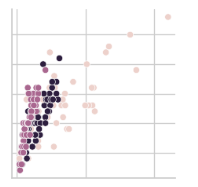
\includegraphics[width=5cm, height=5cm]{Tareas_tiempotareas.png} % Inserta la imagen 
    \caption{Par\'ametro$ = $tareas} % Agrega un título a la imagen 
    \label{fig:mi_imagen4} % Etiqueta para referenciar la imagen en el texto 
\end{figure}

\begin{figure}[H] % ht indica que la figura puede ir "aquí" o en la "parte superior" 
    \centering % Centra la imagen en la página 
    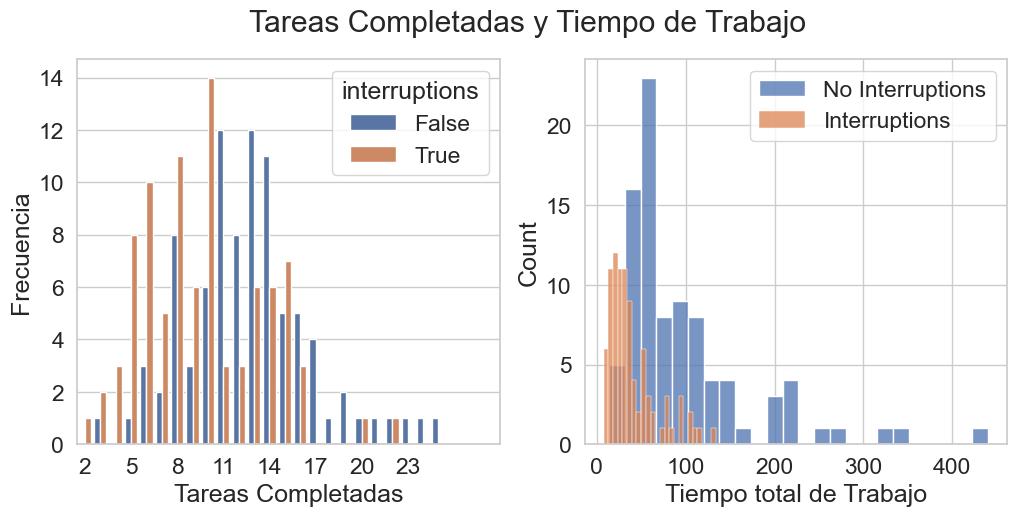
\includegraphics[width=5cm, height=5cm]{tareas_interrupciones.png} % Inserta la imagen 
    \caption{Par\'ametro$ = $tareas} % Agrega un título a la imagen 
    \label{fig:mi_imagen5} % Etiqueta para referenciar la imagen en el texto 
\end{figure}


Como principal resultado obtenido tenemos que no es importante la metodología seguida con respecto a los descansos, se puede ser libre con el horario, el tiempo de trabajo distribuye exponencial y la cantidad de tareas distribuye poisson. Salen a resaltar otros resultados que eran evidentes tales como: el tiempo de trabajo y la cantidad de tareas son proporcionales ~\ref{fig:mi_imagen4} y la cantidad de tareas realizadas se ve afectadas si se simula alguien propenso a interrupciones . Se llevaron a cabo simulaciones de $480$ minutos ($8$ horas) con distintas metodologías, descansos cada $24$, $12$, o una cantidad aleatoria de minutos siguiendo una distribuci\'on exponcial con par\'ametro $\lambda = 24$, la duración de los descanso respectivamente queda : $6$, $3$, o una ~\ref{fig:mi_imagen5}cantidad aleatoria de minutos dada por una distribuci\'on exponencial con par\'ametro $\lambda = 6$; todas estas variaciones se simularon con o sin interrupciones. A partir de las simulaciones con el modelo de colas, se recopilan los datos para conformar el modelo de cadenas de Markov, con el cual se llevan a cabo comparaciones en forma de funci\'on diferencia entre ambos modelos. Se llevan a cabo test para validar las hip\'otesis, entre estos se encuentran: "KS statistic", "Chi-square statistic", "U statistic", "D statistic", "H statistic"; son utilizados para confirmar algunas de nuestras hip\'otesis con alto grado de confianza. Para el criterio de parada se usa que tanto se aleja el estimador muestral del la poblaci\'on, y esto se comprueba cuando $\frac{\sigma}{\sqrt{k}} < c$ donde $c$ es el error que se est\'a dispuesto a cometer(la mitad de la longitud de confianza) con $95\%$ de confianza. 

\subsection{Modelo Matem\'atico}

El modelo esta conformado por un conjunto de estados y transiciones entre estos con ciertos valores, o sea un grafo dirigido ponderado. Se plantean los estados $\{trabajando = W, descansando = B, interrumpido = I\}$, con funci\'on de transici\'on $\delta(q_i) = \{(q_0, p_0), (q_1, p_1), (q_2, p_2)\}$ donde $p_j$ representa la probabilidad de que estando en $q_i$ se vaya a $q_j$.

Se toman un conjunto de restricciones y supuestos de forma severa: No se est\'a en dos estados a la vez, cuando se entra a un estado no se sale hasta que se termina, no se depende de informaci\'on anterior para determinar el estado siguiente, la suma de las probabilidades que salen de un estado suman $1$.

Para el c\'alculo de las probabilidades, se utiliza la probabilidad cl\'asica tomando en cuenta los datos que brindo el modelo basado en teor\'ia de colas. Se cuentan la cantidad de transiciones de estar en el estado $q_i$ hacia el estado $q_j$ denotemosla como $c_j$ entonces, $p_j = \frac{c_j}{\sum_{i=1}^{3} c_i}$.

De antemano es notable que las restricciones tomadas son muy fuertes por lo que los resultados no deber\'ian ser muy justos. Llevamos a cabo varias comparaciones, dada la representaci\'on como cadena de markov, se conto la cantidad de veces que se estaba en cada estado, para simulaciones tomando como entrada la cantidad de iteraciones; por su contrapuesto tenemos al modelo por colas y se quiere ver que tan pr\'oximo resulta la cadena a este, entonces tomamos como aproximaci\'on para cada parametro a $\frac{Tiempo_{parametro}}{cantidad_{parametro}}$ o sea el tiempo que est\'a en los diferentes estados dividido por la cantidad de veces que se complete dicho estado.

Para todas las gr\'aficas se toma como las rojas a la realizada por teor\'ia
de colas, y a la azul a la realizada por cadena de markov.

\begin{figure}[H] % ht indica que la figura puede ir "aquí" o en la "parte superior" 
    \centering % Centra la imagen en la página 
    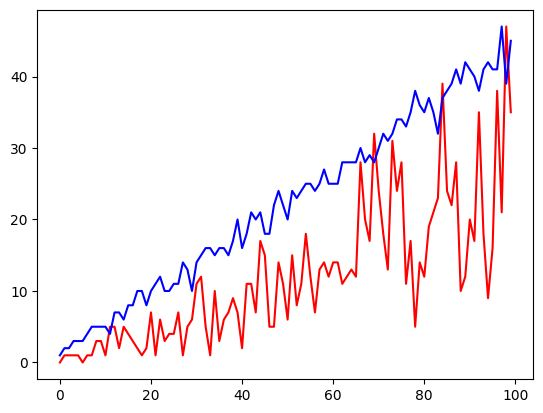
\includegraphics[width=5cm, height=5cm]{comparacion1.jpg} % Inserta la imagen 
    \caption{Par\'ametro$ = $tareas} % Agrega un título a la imagen 
    \label{fig:mi_imagen1} % Etiqueta para referenciar la imagen en el texto 
\end{figure}

\begin{figure}[H] % Otra figura centrada 
    \centering 
    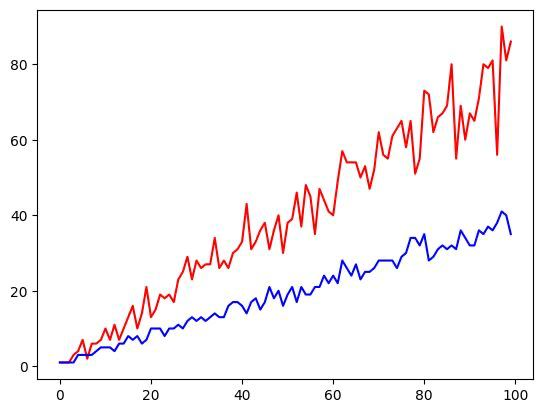
\includegraphics[width=5cm, height=5cm]{comparacion2.jpg} 
    \caption{Par\'ametro$ = $descansos} 
    \label{fig:mi_imagen2} 
\end{figure}

\begin{figure}[H] % Y otra más 
    \centering 
    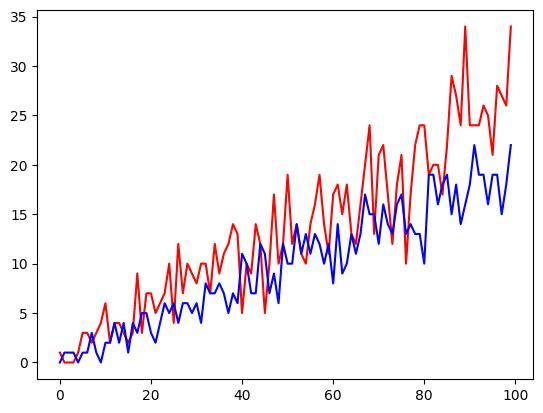
\includegraphics[width=5cm, height=5cm]{comparacion3.jpg} 
    \caption{Par\'ametro$ = $interrupciones} 
    \label{fig:mi_imagen3} 
\end{figure}

\subsubsection*{Comparaciones}
Notemos que aunque se ven diferentes guardan relaci\'on, pues siguen su crecimiento a lo largo del tiempo aunque con un alto grado de ruido en particular cuando se trata de las tareas ~\ref{fig:mi_imagen1}, pues recordemos que se tomo ciertas asunciones con respecto a estas, veamos como con las interrupciones~\ref{fig:mi_imagen3} si se tiene m\'as proximidad porque su comportamiento en ambos modelos es bastante similar 

\begin{thebibliography}{9} 
    \bibitem{ref1} Biwer, F., Wiradhany, W., oude Egbrink, M. G. A., \& de Bruin, A. B. H. 
    (2023).
    \textit{Understanding effort regulation: Comparing ‘Pomodoro’ breaks and self-regulated breaks.}. British Journal of Educational Psychology, 93(Suppl. 2), 353-367. \href{https://doi.org/10.1111/bjep.12593}{https://doi.org/10.1111/bjep.12593}


    \bibitem{ref2} L\'eon G. Faber, Natasha M. Maurits, Monicque M. Lorist. 
    \textit{Mental Fatigue Affects Visual Selective Attention}. Article  in  PLOS ONE · October 2012 
    \href{DOI:10.1371/journal.pone.0048073}{DOI:10.1371/journal.pone.0048073}

    \bibitem{ref1} Blaz Kos. 
    \textit{Interruptions at work Why are they a problem and the best ways to handle them}. 
    Spica.
    \href{https://www.spica.com/blog/interruptions-at-work}{https://www.spica.com/blog/interruptions-at-work}

    \bibitem{ref1} Hannah Ross. 
    \textit{The Impact of Interruptions on Productivity \& How to Combat Them}.
    Fellow.
    \href{https://fellow.app/blog/productivity/the-impact-of-interruptions-on-productivity-how-to-combat-them/}{https://fellow.app/blog/productivity/the-impact-of-interruptions-on-productivity-how-to-combat-them/}

\end{thebibliography}

\end{document} $